%-----------------------------------------------------------------------------%
\chapter{LANDASAN TEORI}
%-----------------------------------------------------------------------------%
\vspace{4.5pt}
Pada bab ini menjelaskan beberapa teori dan jurnal yang berhubungan dengan permasalahan penelitian yang digunakan pada proses penelitian.
\section{Tinjauan Pustaka}
Pembahasan mengenai teori-teori tersebut dijelaskan sebagai berikut.
\subsection{Monolitik}
Monolitik yaitu suatu cara untuk melakukan penyebaran. Ketika semua fungsi dalam sistem harus disebarkan secara bersama-sama, maka itu merupakan sebuah monolitik \cite{74C}. Monolitik merupakan sebuah aplikasi perangkat lunak di mana setiap modulnya tidak bisa dieksekusi secara independen. Hal ini membuat monolitik sulit digunakan pada sistem terdistribusi tanpa bantuan penggunaan \textit{frameworks} atau solusi \textit{ad hoc} seperti Objek Jaringan, \textit{RMI} atau \textit{CORBA} \cite{0BD}.

Penggunaan pada bahasa pemrograman seperti \textit{Java},\textit{C/C++}, dan \textit{Python} pada pengembangan aplikasi di sisi \textit{server}, memiliki kemampuan dalam melakukan abstraksi untuk memecah kompleksitas program menjadi berupa modul. Namun, bahasa pemrograman ini dirancang untuk membuat \textit{artefacts} monolitik. Di mana abstraksi ini tergantung pada penggunaan berbagi sumber data pada komputer yang sama (memori, \textit{database}, \textit{file}) \cite{0BD}.

\subsubsection{Jenis Monolitik}
Setidaknya terdapat 3 jenis monolitik yang memiliki struktur yang berbeda masing-masing namun masih merupakan arsitektur monolitik \cite{74C}:
\begin{enumerate}[leftmargin=1.3cm]
\item \textit{Single Process Monolith}\\
Di mana sebuah kode disebarkan dengan satu proses. Setiap kode bisa berada di banyak \textit{instances} serta tempat penyimpanan dan mendapatkan data disimpan pada suatu \textit{database} yang sama. Variasi lainnya yaitu modular monolitik di mana setiap kode bisa bekerja secara independen tetapi perlu dijadikan satu kesatuan ketika ingin dilakukan \textit{deployment}.
\begin{center}
	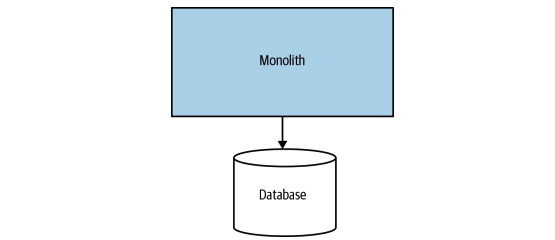
\includegraphics[width=12cm]{img/bab_2/sp_mono.png}
	\captionof{figure}{
	Arsitektur \textit{Single Process Monolith} \cite{74C} }
	\label{fig:msa}
\end{center}
\item \textit{Distributed Monolith}\\
Monolitik terdistribusi adalah sistem yang terdiri dari beberapa layanan, tetapi untuk apa pun alasannya seluruh sistem harus disebarkan bersama-sama. Sebuah monolitik terdistribusi bisa memiliki kesamaan dengan \textit{service-oriented architecture (SOA)}.

Monolitik terdistribusi biasanya muncul  di kondisi di mana tidak cukup fokus pada konsep \textit{information hiding} dan \textit{cohesion} dari fungsi bisnis. Akibatnya terbentuklah arsitektur yang memiliki \textit{coupling} yang tinggi, di mana bisa perubahan menyebabkan kerusakan pada bagian sistem lain.
\item \textit{Sistem Black-Box Pihak Ketiga}\\
Aplikasi pihak ketiga merupakan sebuah monolitik, misalkan sistem penggajian, sistem CRM, dan sistem SDM. Faktor umum yang terjadi yaitu aplikasi ini dibuat dan dikelola oleh orang lain di mana pengembang belum tentu memiliki kemampuan untuk mengubah kode seperti \textit{Software-as-a-Service(SaaS)}.
\end{enumerate}

\subsubsection{Keuntungan} 
Masing-masing jenis monolitik memiliki keuntungan yang sama seperti \cite{ECD,1C7}:
\begin{enumerate}[leftmargin=1.3cm]
\item Sederhana dalam melakukan pengembangan karena \textit{Integrated Development Environment (IDE)} dan peralatan pengembang berfokus pada membuat satu aplikasi
\item Mudah untuk melakukan perubahan secara radikal di aplikasi. Perubahan ini bisa dari kode hingga skema \textit{database} serta proses \textit{deployment}.
\item Pengujian dilakukan pada satu aplikasi, pengembang dapat membuat pengujian dari awal hingga akhir dengan lebih mudah dan terintegrasi
\item \textit{Deployment} dilakukan pada satu aplikasi, pengembang hanya menyalin aplikasi dari komputer ke komputer yang lain. Dengan ini aplikasi relatif mudah dilakukan konfigurasi dan mudah diperbanyak jumlah aplikasi.
\end{enumerate}

\subsubsection{Tantangan} 
Masing-masing jenis monolitik memiliki tantangan yang sama seperti \cite{ECD,1C7}:
\begin{enumerate}[leftmargin=1.3cm]
	\item Sulit dikembangkan secara berkelanjutan, karena semakin banyak orang yang bekerja pada aplikasi yang sama. Akibatnya setiap pengembang memiliki kepentingan masing-masing dalam mengelola kode yang sama dan membuat pengambilan keputusan sulit serta tidak fleksibel
	\item Memiliki reliabilitas yang rendah, karena kesalahan pada salah satu modul aplikasi bisa menyebabkan kegagalan secara keseluruhan aplikasi. Akibatnya aplikasi tidak dapat digunakan oleh pengguna dan harus dilakukan \textit{deployment} kembali.
	\item Tidak mudah untuk melakukan skalabilitas, setiap modul aplikasi memiliki kebutuhan sumber daya yang berbeda seperti ada modul penyediaan data yang membutuhkan banyak memori sedangkan modul pemrosesan gambar membutuhkan banyak CPU, karena modul ini berada pada aplikasi yang sama akibatnya pengembang harus melakukan pengorbanan pada salah satu sisi sumber daya.
	\item Terkunci pada teknologi lama, pengembang terkunci pada teknologi awal yang digunakan untuk membangun aplikasi. Pengembang juga kesulitan ketika ingin mengadopsi teknologi baru pada aplikasi karena sangat berisiko dan sangat mahal untuk menulis kembali seluruh aplikasi antar teknologi.\\
\end{enumerate}	

\subsection{\textit{Microservice}}
\textit{Microservice} adalah beberapa \textit{service} yang bisa di\textit{deploy} secara independen yang dimodelkan berdasarkan bisnis domain. \textit{Service} ini berkomunikasi satu sama lain melalui jaringan komputer dan bisa dibangun dengan berbagai macam teknologi. \textit{Microservice} adalah salah tipe dari \textit{service oriented architecture (SOA)} meskipun ada perbedaan dalam membuat batasan antara \textit{service} dan \textit{deployment} secara independen \cite{74C}.

\textit{Service} adalah komponen perangkat lunak yang memiliki kegunaannya secara khusus di mana komponen ini bisa berdiri sendiri dan secara independen dilakukan proses \textit{deployment}. Service memiliki \textit{API (Application Programming Interface)} yang memberikan akses kepada \textit{client} untuk melakukan operasi. Terdapat 2 tipe operasi yaitu perintah dan \textit{query}.
\textit{API} terdiri dari perintah, \textit{query} dan \textit{event}. Perintah dapat berupa \textit{buatPesanan()} yang melakukan aksi dan memperbarui data. \textit{Query} dapat berupa \textit{cariPesananBerdasarkanID()} yang digunakan untuk mengambil data. \textit{Service} juga dapat membuat suatu \textit{event} seperti \textit{PesananSudahDibuat} di mana \textit{event} ini akan dikonsumsi oleh \textit{client}-nya / \textit{subscriber} \cite{1C7}.

\begin{center}
	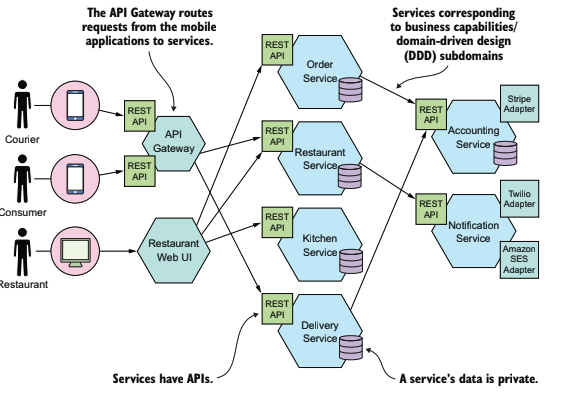
\includegraphics[width=12cm]{img/bab_2/micro_arch.png}
	\captionof{figure}{
	Arsitektur \textit{Microservice} \cite{1C7} }
	\label{fig:msa}
\end{center}

\textit{Service API} akan mengenkapsulasi internal implementasinya, sehingga pengembang aplikasi tidak bisa menuliskan kode yang melewati \textit{API}. Akibatnya arsitektur \textit{microservice} dapat mewajibkan modularitas di aplikasi.  Setiap \textit{service} di arsitektur \textit{microservice} memiliki masing-masing arsitektur sendiri dan dimungkinkan dengan teknologi yang berbeda. Tetapi kebanyakan \textit{service} memiliki arsitektur heksagonal. Di mana \textit{API} akan diimplementasi melalui adapter yang berinteraksi dengan logika bisnis \cite{1C7}

\subsubsection{Ciri Khusus \textit{Microservice}}
Hal yang membedakan arsitektur \textit{microservice} dengan arsitektur lainnya yaitu \cite{ECD,74C,1C7}:	
\begin{enumerate}[leftmargin=1.3cm]
	\item Kecil dan berfokus pada satu hal dengan baik\\
	\textit{Service} yang dibuat memiliki \textit{encapsulation} dengan pembuatan \textit{service} dimodelkan di sekitar Domain Bisnis, tujuannya agar ketika terjadi perubahan antar \textit{service} bisa dilakukan dengan lebih mudah dan tidak berdampak pada \textit{service} lain. Oleh karena itu \textit{service} yang dibuat seminimal mungkin untuk tidak berhubungan dengan \textit{service} lain. 
	\item Otonomi / Bisa berdiri sendiri\\
	\textit{Microservice} memiliki \textit{service} yang terisolasi di mana bisa memiliki sistem operasi hingga komputer yang berbeda. Dengan ini sistem terdistribusi lebih sederhana dan nilai \textit{coupling} yang rendah. Semua komunikasi antar \textit{service} dilakukan melalui jaringan sehingga \textit{service} harus memiliki kemampuan di\textit{deploy} sendiri tanpa harus mempengaruhi \textit{service} lain.
	\item Data yang dikelola masing-masing \textit{service}\\
	\textit{Service} yang membutuhkan data di luar domainnya harus berkomunikasi melalui \textit{API(application programming interface)}, dengan ini setiap \textit{service} memiliki tanggung jawab terhadap datanya masing-masing sehingga data tersebut hanya bisa diubah oleh \textit{service} itu sendiri. Setiap \textit{service} memiliki data yang pribadi dan data yang bisa dibagikan kepada \textit{service} lain
\end{enumerate}	

\subsubsection{Keuntungan}
Keuntungan dari menggunakan arsitektur \textit{Microservice}  \cite{ECD,74C,1C7}:
\begin{enumerate}[leftmargin=1.3cm]
	\item Memudahkan pengembangan aplikasi kompleks dan fleksibel\\
	\textit{Service} berukuran kecil sehingga mudah dikelola, perubahan pada satu \textit{service} bisa diterapkan secara independen dari \textit{service} lainnya. Bila terjadi kegagalan di satu \textit{service} tidak berdampak besar pada \textit{service} lainnya karena \textit{service} masing-masing terisolasi selain itu proses pemulihan bisa dilakukan dengan mudah dan cepat.
	\item Bisa dilakukan \textit{scaling} secara independen\\ 
	Setiap \textit{service} memiliki fungsi yang berfokus pada satu hal,  di mana setiap \textit{service} bisa memiliki kebutuhan sumber daya berbeda. Penggunaan sumber daya ini bisa dikelola dengan mudah dan cepat karena setiap \textit{service} dapat di\textit{deploy} dengan jumlah \textit{service} yang berbeda.
	\item Mudah melakukan percobaan dan penggunaan teknologi baru\\
	Arsitektur \textit{microservice} mengeliminasi komitmen penggunaan secara lama pada suatu teknologi. Dengan ini pengembang dapat memilih berbagai teknologi dalam membangun \textit{service} serta \textit{service} yang kecil dan berfokus lebih mudah untuk dilakukan migrasi antara teknologi yang berbeda. 
\end{enumerate}	

\subsubsection{Tantangan}
Tantangan dari menggunakan arsitektur \textit{Microservice}  \cite{ECD,74C,1C7}:
\begin{enumerate}[leftmargin=1.3cm]
	\item Menemukan \textit{service} yang tepat itu sulit\\
	Salah satu tantang terbesar dari membuat \textit{microservice} yaitu tidak adanya cara yang pasti bagaimana untuk melakukan dekomposisi dengan baik. Di mana \textit{service} yang didekomposisi dengan tepat tidak mudah ditemukan dan bila dilakukan dengan tidak benar dapat sebaliknya membuat \textit{distributed monolith}. 
	\item Memiliki kompleksitas karena merupakan suatu terdistribusi\\
	Setiap \textit{service} untuk berkomunikasi antar \textit{service} memiliki tantangan masing-masing seperti latensi, konsistensi data, dan kondisi ketika beberapa \textit{service} mengalami kegagalan. \textit{Microservice} juga meningkatkan kompleksitas operasional oleh karena itu untuk melakukan \textit{deployment} sebaiknya menggunakan proses otomatisasi.
	\item \textit{Deployment} yang melibatkan beberapa service\\
	Untuk melakukan \textit{deployment} ini dibutuhkan koordinasi antara tim pengembang \textit{servic} ketika menambahkan atau mengubah fitur yang berdampak pada beberapa \textit{service} maka dari itu harus dibuat perencanaan \textit{deployment} berdasarkan ketergantungan antar \textit{service}.
\end{enumerate}	

\subsubsection{Permasalahan dan Pola penyelesaiannya}
Arsitektur \textit{Microservice} memiliki banyak hal yang harus dipertimbangkan oleh karena itu dibutuhkan strategi dan pola untuk menyelesaikan suatu masalah yang dapat terjadi dalam penerapan arsitektur \textit{microservice} \cite{1C7}:
\begin{center}
	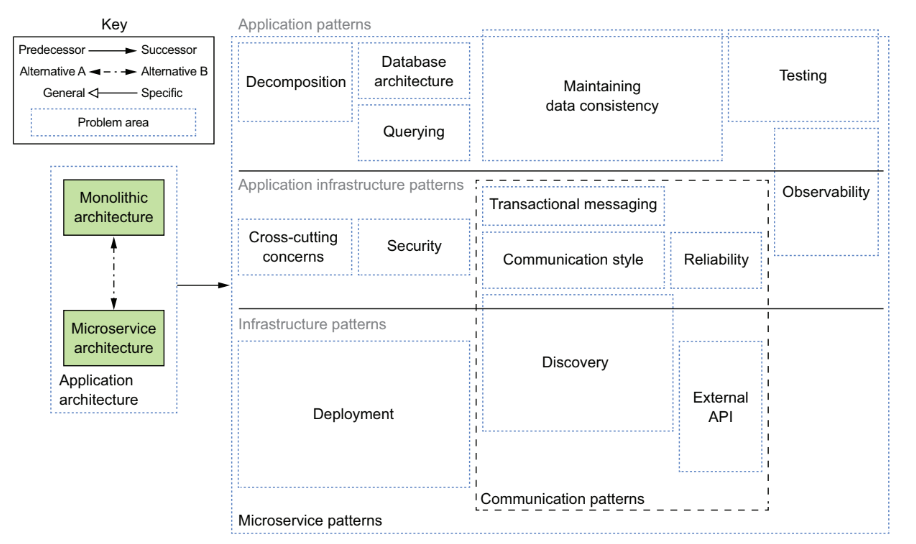
\includegraphics[width=12cm]{img/PolaMicroservice.png}
	\captionof{figure}{
	Pola dalam menyelesaikan masalah di arsitektur \textit{Microservice} \cite{1C7} }
	\label{fig:msa}
\end{center}
\begin{enumerate}[leftmargin=1.3cm]
	\item \textit{Application patterns}\\
	Permasalahan yang harus diselesaikan oleh pengembang aplikasi, yaitu bagaimana cara dekomposisi sistem menjadi beberapa \textit{service}. Terdapat beberapa Strategi yang dapat dilakukan seperti berdasarkan sub-domain dan berdasarkan proses bisnis. Service mengelola datanya masing-masing namun ini menyebabkan permasalahan tersendiri karena bisa terjadi data yang tidak konsisten antara \textit{service}. Pendekatan biasa seperti 2PC tidak cocok pada aplikasi modern sehingga konsistensi data dicapai melalui SAGA.
	
	Perbedaan penyimpanan data membuat \textit{query} harus menggabungkan data yang dimiliki oleh beberapa \textit{service} yang terlibat karena data hanya bisa diakses melalui API. Terkadang bisa digunakan komposisi API di mana memanggil API \textit{service} satu dengan yang lain atau dengan \textit{Command Query Responsibility Seqgregation(CQRS)} yaitu ketika setiap \textit{service} memiliki replika data dari \textit{service} yang dibutuhkan.

	Pengujian pada \textit{service} mudah dilakukan karena memiliki lingkup yang kecil dan terpusat namun untuk menguji beberapa \textit{service} tidak mudah, karena banyaknya proses yang harus dilakukan. Sehingga diperlukan proses otomatisasi proses pengujian. Ada beberapa pola yang dapat digunakan untuk pengujian di \textit{microservice} yaitu pengujian dilakukan pada \textit{client}, pengujian pencocokan pada \textit{client}, dan pengujian secara terisolasi.  

	\item \textit{Application infrastructure} \\
	Permasalahan infrastruktur yang memiliki pengaruh pada proses pengembangan aplikasi. Aplikasi yang dibangun dengan \textit{microservice} merupakan sistem terdistribusi. Sehingga komunikasi antar proses adalah bagian yang penting dapat arsitektur \textit{microservice}. Diperlukan variasi arsitektur dan keputusan desain tentang bagaimana \textit{service} berkomunikasi satu dengan yang lain. 

	Pola komunikasi dikelompokkan menjadi 5 grup yaitu gaya komunikasi, \textit{discovery} reliabilitas, \textit{Transactional Messaging}, API Eksternal. Terdapat 3 gaya komunikasi yaitu \textit{Messaging} di mana komunikasi dapat dilakukan secara \textit{asynchronous}, \textit{Domain-Specific} di mana komunikasi harus melalui protokol tertentu seperti Email, dan \textit{Remote Procedure Invocation}(RPI) di mana komunikasi dilakukan secara \textit{asynchronous}.
	
	Cara \textit{Messaging} memiliki kelemahan karena transaksi terdistribusi tidak cocok digunakan pada aplikasi modern untuk mengatasi ini ada 2 pendekatan yaitu \textit{polling publisher} di mana menggunakan tabel OUTBOX untuk menyimpan message sementara dan Log Tailing di mana melihat transaksi terakhir dari message.

	Ketika \textit{service} sedang berkomunikasi dan waktu menunggu jawaban dari \textit{service} lain melebihi batas yang ditentukan maka bisa terjadi kemungkinan \textit{service} tersebut mengalami kegagalan. Pola Circuit Breaker dapat diterapkan bila terjadi hal seperti ini tujuannya agar \textit{service} tidak berkomunikasi pada \textit{service} yang gagal.

	Pada arsitektur \textit{microservice} untuk proses authentikasi pengguna umumnya dilakukan oleh \textit{API Gateway}. Di mana \textit{API Gateway} melanjutkan informasi ke \textit{service} yang bertanggung jawab mengenai authentikasi, solusi umumnya yaitu menggunakan Access Token seperti JWT(JSON Web Token).
	\item \textit{Infrastructure patterns}\\
	Permasalahan infrastruktur yang muncul diluar dari pengembangan aplikasi. Infrastruktur menangani proses\textit{deployment}, discovery, dan External API. 
	Discovery adalah bagaimana \textit{service} bisa ditemukan agar bisa berkomunikasi, terdapat beberapa pendekatan yang bisa dilakukan seperti \textit{service} ditemukan dari \textit{client} atau dari server dan proses registrasi bisa dilakukan secara sendiri atau melalui pihak ke-3.

	Eksternal API adalah bagaimana aplikasi pengguna berinteraksi dengan \textit{service}.
	Ada 2 cara untuk aplikasi berinteraksi yaitu \textit{API Gateway} dan \textit{Backend for Frontend}. Proses \textit{Deployment} \textit{microservice} memiliki proses yang kompleks karena \textit{service} yang dikelola bisa berjumlah 10 hingga ratusan \textit{service}, sehingga diperlukan proses otomatisasi yang bisa mengelola \textit{service} dan proses \textit{scaling} bisa diatur berdasarkan kebutuhan. Cara melakukan\textit{deployment} bisa dengan \textit{container}, \textit{virtual machine}, \textit{serverless}, atau menggunakan platform\textit{deployment} \\	
\end{enumerate}	

\subsection{\textit{Enterprise Resource Planning}}
\textit{Enterprise Resource Planning} (ERP) adalah suatu sistem perangkat lunak yang memungkinkan perusahaan untuk mengotomatisasikan dan mengintegrasikan proses bisnisnya dengan komputerisasi. Dengan ini setiap informasi yang diperlukan di proses bisnis dapat dibagikan dan digunakan disemua bagian perusahaan dengan alur terstruktur. Sistem ERP dapat mengeliminasi duplikasi data dan memberikan integrasi data. Sistem ERP memiliki \textit{database} di mana semua transaksi bisnis dapat direkam, diproses, dipantau dan dilaporkan. Tujuannya agar proses bisnis bisa dilakukan dengan lebih cepat, murah, dan transparan \cite{D94}.

Sistem ERP dapat memberikan dukungan untuk proses bisnis perusahaan melalui modul yang terpisah. Setiap modul adalah aplikasi perangkat lunak yang dibangun khusus untuk setiap operasi bisnis. Umumnya modul yang ditemukan pada ERP yaitu Modul Produksi, Modul Manajemen Rantai Pasokan, Modul Keuangan, Modul Penjualan \& Pemasaran, Modul Sumber Daya Manusia, dan modul pelengkap lainnya seperti \textit{e-commerce} \cite{D94}.

\subsubsection{Arsitektur ERP}
Arsitektur dari sistem ERP dapat didefinisikan menjadi 2 tipe yaitu \textit{logical} dan \textit{physical}. Arsitektur \textit{logical} menggambarkan bagaimana sistem diorganisasikan untuk mendukung kebutuhan bisnis sedangkan arsitektur \textit{physical} mengenai bagian komponen fisik dari keseluruhan sistem untuk melihat performa dan mengurangi biaya. Berikut adalah arsitektur \textit{physical} \cite{D94} 
\begin{enumerate}[leftmargin=1.3cm]
	\item \textit{The Tiered}\\
	Arsitektur \textit{tiered} umumnya dirancang dalam bentuk lapisan yang didasarkan dari model \textit{client-server} atau bisa disebut \textit{N-Tier}. Dalam arsitektur ini setiap komponen ERP disusun ke dalam masing-masing lapisan seperti lapisan \textit{user interface}, lapisan aplikasi dan lapisan \textit{database} / penyimpanan data.
	\item \textit{Web-based}\\
	Arsitektur \textit{Web-based} mengadopsi teknologi berorientasi objek web di mana pengguna yang ingin menggunakan sistem ERP bisa mengakses melalui \textit{browser} dan internet. \textit{Object-oriented technology} diimplementasi untuk mencampur data dan fungsi yang tersedia di berbagai web \textit{service}.
	\item \textit{Service Oriented}\\
	\textit{SOA(Service Oriented Architecture)} adalah sistem yang di mana terdapat fungsi  modular yang berkomunikasi melalui jaringan. Satu atau lebih \textit{service} bisa berkordinasi dalam suatu aktivitas fungsi bisnis. 
	\item \textit{Cloud}\\
	\textit{Cloud} dapat memberikan solusi bagi organisasi ketika mengadopsi sistem ERP pada kegiatan bisnisnya. Sistem ERP dengan arsitektur \textit{cloud} bisa dikategorikan sebagai tipe \textit{SaaS(Software as a Service)}. Organisasi akan membayar pihak ke tiga setiap periode berdasarkan modul yang digunakannya.\\ 
\end{enumerate}

\subsection{Analisis Kode}
Analisis Kode adalah suatu proses mengekstraksi informasi mengenai suatu program dari kode atau artefak. Proses ini bisa dilakukan secara manual yaitu dengan melihat kode program atau bahasa mesin namun kompleksitas program yang tinggi membuat proses secara manual sangat sulit dan tidak efektif. Sehingga diperlukan alat otomatisasi yang dapat membantu proses analisis kode. Alat ini dapat memberikan informasi kepada pengembang mengenai program yang dianalisis \cite{208}. 

\subsubsection{Anatomi} 
Anatomi Analisis Kode yaitu tahapan dan langkah yang harus dilakukan untuk menemukan hasil analisis kode \cite{208}:
\begin{enumerate}[leftmargin=1.3cm]
	\item Ekstraksi Data\\
	Proses ini adalah proses pertama kali dilakukan sebelum melakukan analisis kode, data yang diekstraksi berasal dari kode program. Umumnya dilakukan dengan \textit{syntatic analyzer} atau \textit{parser}. Proses \textit{Parser} ini mengonversi urutan karakter menjadi suatu kata-kata dan mengekstraksi nilai semantik sebenarnya. Tujuannya agar memudahkan proses analisis/transformasi dan penambahan data lainnya.
	\item Representasi Informasi\\
	Proses yang merepresentasikan informasi kode menjadi bentuk yang lebih abstrak. Tujuan dari fase ini untuk membentuk beberapa bagian kode agar terhubung pada analisis secara otomatis. Representasi ini kebanyakan berupa \textit{graph} seperti \textit{Abstract Syntax Trees (AST)}, \textit{Control Flow Graphs (CFG)}, dan \textit{Call Graph}.
	\item Eksplorasi Pengetahuan\\
	Setelah informasi direpresentasikan, informasi dibuat menjadi suatu kesimpulan. Kesimpulan bisa dibuat secara kuantitatif atau kualitatif, proses visualisasi penting dalam proses eksplorasi pengetahuan kode program.
\end{enumerate}

\subsubsection{Strategi Analisis}
Terdapat berbagai cara dan pertimbangan dalam melakukan analisis kode \cite{208}:
\begin{enumerate}[leftmargin=1.3cm]
	\item Statik vs Dinamis\\
	Analisis secara statik menganalisis program tanpa dieksekusi untuk mendapatkan semua informasi yang kemungkinan akan dieksekusi. Sedangkan secara Dinamis, program mengumpulkan informasi yang dieksekusi dengan nilai yang diberikan. Beberapa teknik analisis menggabungkan kedua pendekatan ini.
	\item \textit{Sound vs Unsound}\\
	\textit{Sound} yaitu analisis yang bisa menjamin secara keseluruhan dan kebenaran eksekusi program. Sedangkan \textit{Unsound} tidak bisa secara keseluruhan menjaminkan kebenaran hasil analisis program. Namun dalam banyak kasus analisis \textit{Unsound} memiliki hasil yang benar selain itu memiliki kelebihan yaitu mudah diimplementasi dan efisien.
	\item \textit{Flow sensitive vs Flow insensitive}\\
	\textit{Flow sensitive} memperhatikan dan menyimpan urutan proses eksekusi sedangkan \textit{Flow insensitive} tidak memperhatikan urutan proses eksekusi sehingga tidak memiliki informasi ketergantungan pada suatu proses dan hanya dapat menyatakan proses tersebut ada.
	\item \textit{Context sensitive vs Context insensitive}\\
	\textit{Context in-sensitive} hanya menghasilkan satu hasil yang berhubungan dalam semua konteks. Sedangkan \textit{context sensitive} memiliki hasil berbeda ketika konteks berbeda. Pendekatan ini bertujuan untuk menganalisis proses pembuatan analisis umumnya tanpa adanya informasi mengenai konteks yang akan digunakan. \textit{Context sensitive} penting untuk menganalisis program modern di mana terdapat suatu abstraksi.
\end{enumerate}

\subsubsection{Tantangan}
Untuk melakukan kode analisis terdapat tantangan dan kesulitan untuk mendapatkan hasil analisis yang sempurna \cite{208}:
\begin{enumerate}[leftmargin=1.3cm]
	\item Perbedaan bahasa kode program\\
	Banyak peningkatan dan perubahan pada bahasa pemrograman seperti \textit{dynamic class loading} dan \textit{reflection}. Konsep ini juga terdapat pada proses pengubahan tipe data, \textit{pointer}, \textit{Anonymous types} yang membuat proses \textit{parser} sulit. Fitur pada pemrograman ini meningkatkan fleksibilitas ketika program berjalan dan membutuhkan analisis secara dinamik yang lebih kuat.
	\item \textit{Multi-Language}\\
	Banyak aplikasi yang dibuat sekarang dibangun dengan berbagai bahasa pemrograman. Di mana sekarang perlengkapan pembuatan aplikasi masih belum bisa menganalisis secara keseluruhan pada aplikasi yang menggunakan banyak bahasa pemrograman. Seperti aplikasi berbasis web yang memiliki \textit{HTML}, \textit{ASP}, \textit{Java} dan lainnya.
	\item Analisis secara \textit{Real-Time}\\
	Analisis ini dapat memberikan keuntungan bagi pengembang karena memberikan informasi tambahan selama pengembang membuat aplikasi seperti \textit{code coverage} dan analisis kebocoran memori. Proses analisis juga kerap kali membutuhkan penggunaan sumber daya komputasi yang tinggi dan memori yang banyak.\\
\end{enumerate}

\subsection{Dekomposisi}
Dekomposisi merupakan proses pemisahan bagian dari aplikasi, proses dekomposisi sendiri dapat menyebabkan masalah dengan latensi, penyelesaian masalah, integritas, kegagalan bersamaan, dan hal lainnya. 

\subsubsection{Pemilihan Bagian yang didekomposisi}
Terdapat beberapa cara untuk melakukan dekomposisi aplikasi monolitik, dekomposisi ini menentukan bagaimana bagian aplikasi menjadi \textit{Service}:
\begin{enumerate}[leftmargin=1.3cm]
	\item Kemampuan Bisnis\cite{1C7}\\
		 Service dibuat dari pendekatan proses arsitektur bisnis di mana setiap kegiatan bisnis memiliki ketergantungan terhadap kegiatan bisnis lainnya. Contohnya Toko Online memiliki hubungan dengan proses pemesanan, penyimpanan barang, pengiriman dan lainnya. Untuk menemukan kemampuan bisnis bisa dianalisis dari tujuan organisasi, struktur organisasi dan proses bisnisnya. Setiap kemampuan bisnis bisa dianggap sebagai suatu \textit{service}.

		 Kemampuan bisnis juga sering berfokus pada objek bisnis, seperti berfokus pada  setiap hal masukan, hasil, dan perjanjian. Kemampuan bisnis bisa memiliki bagian kecil lainnya. bagian kecil lainnya terkadang bisa merepresentasikan hal yang sangat berbeda.
	\item \textit{Domain Driver Design} (DDD) \cite{1C7} \\
		DDD mengambil konsep mencari domain di mana domain tersebut dapat digunakan untuk menyelesaikan permasalahan di dalam domain itu sendiri. Model domain hampir mencerminkan antara desain dan implementasi aplikasi. DDD memiliki 2 konsep yang sangat penting saat mengimplementasikan di arsitektur \textit{microservice} yaitu subdomain dan \textit{bounded context}.

		DDD memisahkan domain model untuk setiap subdomainya, subdomain adalah bagian dari doamin. Subdomain diidentifikasi melalui pendekatan yang sama dengan mencari kemampuan bisnis. DDD menggunakan \textit{bounded context} dalam menentukan batasan suatu domain, \textit{bounded context} termasuk kode yang mengimplementasikan model. Pada \textit{microservice} \textit{bounded context} bisa berupa satu \textit{service} atau beberapa kumpulan \textit{service}.
	\item Analisis Kode \cite{74C,5B1}  \\
		Transformasi aplikasi monolitik menjadi \textit{microservice} bisa dilakukan dengan strategi analisis statik atau dinamis. Umumnya hal yang perhatikan adalah ketergantungan / keterhubungan antar module, kemudian menerapkan proses clustering atau algoritma evolusi pada ketergantungan module untuk menghasilkan partisi-partisi module yang sudah ditentukan dari evaluasi tertentu seperti nilai \textit{coupling} yang rendah dan nilai \textit{cohesion} yang tinggi. Analisis ini sendiri bisa berupa campuran antara proses bisnis dekomposisi secara fungsional, \textit{control flow}, \textit{data flow}, dan \textit{semantic model}
		
\end{enumerate}	

Untuk menentukan batasan \textit{microservice} perlu diketahui bagaimana struktur kode mempengaruhi secara \textit{coupling} dan \textit{cohesion}. \textit{Coupling} berfokus pada bagaimana perubahan pada satu hal membuat bagian lain mengalami perubahan. \textit{Cohesion} berfokus pada bagaimana kode dikelompokkan satu sama lain \cite{74C}. 

Struktur Microservice yang ideal memiliki \textit{cohesion} yang tinggi dan \textit{coupling} yang rendah, karena dengan \textit{cohesion} yang tinggi setiap \textit{service} memiliki fokusnya masing-masing dan perubahan dilakukan pada spesifik \textit{service} sedangkan dengan \textit{coupling} rendah membuat \textit{service} bisa berdiri sendiri / independen dan setiap \textit{service} mungkin tidak harus sering berinteraksi satu sama lain \cite{74C}.

\textit{Coupling} merupakan tentang bagaimana bagian yang terhubung memiliki dampak satu sama lain, ketika satu \textit{service} berubah dan \textit{service} itu dihubungkan dengan banyak \textit{service} maka  \textit{service} lainnya harus beradaptasi terhadap perubahan tersebut. Terdapat beberapa tipe \textit{coupling} seperti  \textit{Logical Coupling},  \textit{Temporal Coupling},  \textit{Deployment Coupling}, dan  \textit{Domain Coupling}.

\textit{Cohesion} merupakan tentang bagaimana kode yang dikelompokkan bersama adalah kode yang memiliki keterhubungan kuat. Sehingga ketika terjadi perubahan pada satu bagian, bagian yang lain diubah bersama-sama. Pengelompokan kode yang tepat dapat membantu pengembang untuk melakukan perubahan ketika diperlukan tanpa harus mengganggu stabilitas sistem secara keseluruhan.

\subsubsection{Permasalahan dan Pola Penyelesaiannya}
Ketika sudah menentukan \textit{service} yang ingin didekomposisi diperlukan pola dan strategi untuk memisahkan bagian yang ingin didekomposisi. Setiap pola memiliki kekurangan dan kelebihannya masing-masing \cite{74C}:
\begin{enumerate}[leftmargin=1.3cm]
	\item Pola \textit{Strangle} \textit{Fig} \\
		  Pola ini terinspirasi cabang yang bisa berdiri sendiri pada pohon, cabang ini awal mulanya adalah bagian besar dari pohon yang lama kelamaan membentuk akarnya sendiri sehingga bisa mendukung kebutuhannya sendiri tanpa harus bergantung pada pohon yang lama.  Ide ini pada pengembangan perangkat lunak yaitu bahwa aplikasi dahulu tetap bisa berjalan bersamaan dengan aplikasi baru. Aplikasi baru akan tumbuh dan mengambil alih aplikasi dahulu tersebut.

		  \begin{center}
			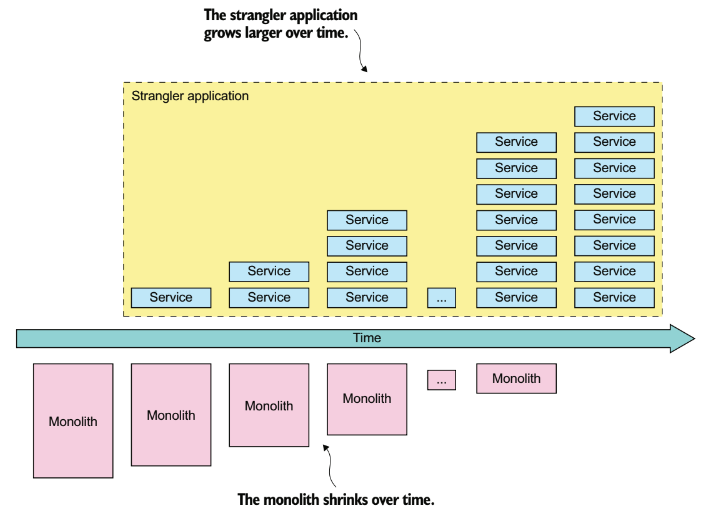
\includegraphics[width=12cm]{img/bab_2/strangle_timeline.png}
			\captionof{figure}{Proses migrasi dari waktu ke waktu}
			\label{fig:asd}
		  \end{center}

		  Terdapat 3 tahap utama dalam menerapkan \textit{strangle} yaitu memilih bagian yang ingin dipindah, memindahkan bagian tersebut menjadi \textit{service} sendiri, dan mengalihkan panggilan pada bagian itu ke \textit{service} yang baru dibuat. Apabila terjadi kegagalan selama migrasi maka sistem bisa dikembalikan seperti semula. Penerapan \textit{strangle} bisa dilakukan untuk memindahkan fitur lama atau pun menambahkan fitur baru.	Untuk mengalihkan panggilan \textit{service} dapat dilakukan melalui \textit{proxy} yang akan merutekan ke \textit{service} yang dapat menangani panggilan tersebut.

		 \begin{center}
			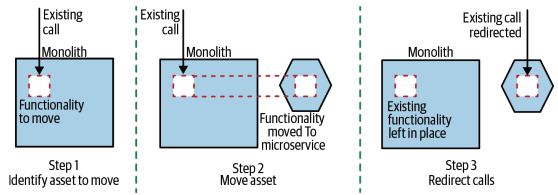
\includegraphics[width=12cm]{img/bab_2/strangle_process.png}
			\captionof{figure}{Proses melakukan \textit{Strangle} \textit{Fig}}
			\label{fig:asd}
		 \end{center}

	\item Pola UI Composition\\
		  Pola ini digunakan pada User Interface(UI), di mana pemecahan dilakukan pada sisi tampilan aplikasi(UI). User Interface akan memanggil beberapa \textit{service} yang dibutuhkannya. Terdapat beberapa pendekatan dalam pemecahan disisi UI yaitu Page Composition, Widget Composition, dan Micro Frontends. Penggunaan pola membutuhkan kode aplikasi user interface bisa dimodifikasi umumnya teknik ini tergantung dari teknologi yang mengimplementasinya.
	\item Branch By Abstraction\\
		  Pola \textit{Strangle} \textit{Fig} dapat dilakukan untuk memindahkan fungsionalitas namun ketika fungsionalitas itu berada di dalam sistem yang lebih dalam. Maka proses ekstraksi harus dilakukan tanpa mempengaruhi banyak sistem di mana sistem lain bisa berubah tanpa diketahui sistem yang diekstraksi. 

		  Branch By Abstraction memiliki 5 tahap yaitu: membuat abstraksi dari fungsi yang akan diubah, mengubah pengguna yang menggunakan fungsi dengan abstraksi yang baru, membuat implementasi baru dari abstraksi, mengubah abstraksi untuk menggunakan implementasi yang baru, membersihkan abstraksi dan menghapus implementasi yang dahulu.

		\begin{figure}[h]
			\centering
			\subfloat[Penggunaan Abstraksi]{
				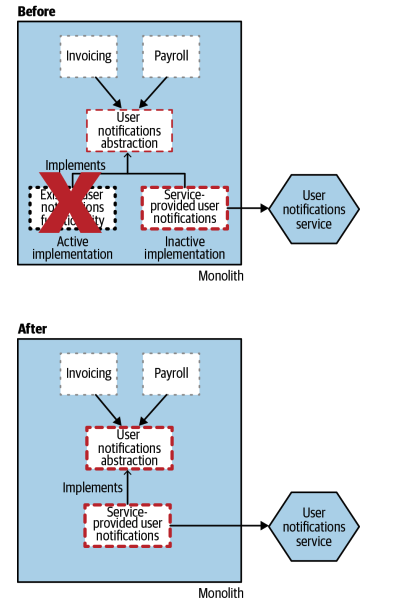
\includegraphics[width=0.45\textwidth]{img/bab_2/abs_imp.png}
				\label{fig:f1}}
			\hfill
			\subfloat[Penggunaan Implementasi Baru]{
				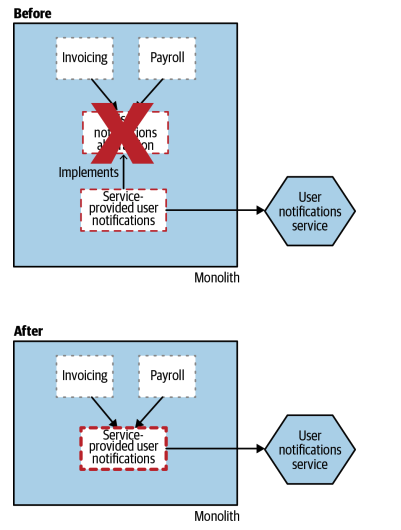
\includegraphics[width=0.45\textwidth]{img/bab_2/abs_clean.png}
				\label{fig:f2}}
			\caption{Ilustrasi Proses Branch By Abstraction}
		\end{figure}
		
	\item Parallel Run\\
		Parallel Run adalah pola bagaimana mengeksekusi sistem yang baru dan sistem yang lama ketika dipisahkan. Teknik ini dapat membuat 2 fungsionalitas di antara sistem baru dan sistem lama dapat berjalan bersama-sama. Hasil dari sistem bisa digunakan sebagai acuan atau verifikasi bahwa sistem baru dapat berjalan dengan benar dan dapat menggantikan sistem lama. Penggunaan metode ini jarang digunakan karena biasanya digunakan pada kasus fungsi yang memiliki risiko tinggi.
	\item Decorating Collaborator\\
		Pola ini digunakan ketika dibutuhkan proses berdasarkan apa yang terjadi di dalam monolitik, tapi pengembang tidak bisa mengubah monolitik itu sendiri. Pola Decorator dapat menambahkan fungsionalitas pada sistem di mana sistem itu sendiri tidak sadar mengenai fungsionalitas tambahan tersebut. Caranya yaitu panggilan langsung ke aplikasi monolitik dan tidak perlu dialihkan tetapi hasil / \textit{response} aplikasi monolitik dialihkan ke \textit{service} yang dapat mengolaborasi hasil tersebut.
	\item Change Data Capture\\
		Change Data Capture tidak menangkap panggilan dan bertindak pada panggilan yang menuju ke monolitik tetapi bereaksi dari perubahan yang terjadi pada penyimpanan data. Untuk mengimplementasikannya yaitu dengan \textit{Database Triggers}, \textit{Transaction Log Pollers}, dan \textit{Batch Delta Copier}. Pola ini dapat digunakan ketika ingin melakukan replikasi data atau proses migrasi data.
\end{enumerate}	

\subsubsection{Tantangan dan Hambatan}
Terdapat tantangan dan hambatan ketika melakukan proses dekomposisi. Tantangan dan hambatan dapat terjadi karena proses dekomposisi itu sendiri \cite{1C7}:
\begin{enumerate}[leftmargin=1.3cm]
	\item Latensi Jaringan\\
		  Latensi jaringan merupakan hal yang dikhawatirkan pada sistem terdistribusi. Beberapa dekomposisi pada \textit{service} dapat menimbulkan tinggi latensi antara dua \textit{service}. Solusi untuk mengatasi permasalahan ini yaitu dengan menggabungkan kedua \textit{service} tersebut atau mengganti proses komunikasi antar \textit{service} tersebut.
	\item Menjaga konsistensi data antar service\\
		  Data yang sebelumnya berada di satu sistem, setelah didekomposisi data tersebar di beberapa \textit{service}. Sehingga proses pengaksesan dan perubahan data lebih rumit. Pada kasus transaksi yang membutuhkan ACID(Atomicity, Consistency, Isolation, and Durability) \textit{microservice} tidak memiliki isolasi karena proses transaksi terjadi tidak hanya di satu \textit{service}.
	\item Adanya God Class yang mencegah dekomposisi\\
		  God Class adalah \textit{class} yang berukuran besar dan berdampak secara luas diaplikasi. Class ini biasanya mempunyai hubungan dengan \textit{class} lainnya dan mengelola berbagai aspek di aplikasi. Solusinya yaitu dengan membuat suatu library dari God Class tersebut dan memecah God Class menjadi \textit{service} yang berfokus pada satu hal. Pendekatan lainnya yaitu dengan DDD di mana dibuat banyak domain dan subdomain.\\
\end{enumerate}	

\subsection{\textit{Clustering}}
\textit{Clustering} yaitu suatu proses untuk melakukan pengelompokan atau klasifikasi objek. Objek bisa ditentukan dari pengukuran atau berdasarkan hubungan antar objek lainnya. Tujuan dari clustering yaitu untuk  menemukan struktur data yang valid. Cluster terdiri dari sejumlah object serupa yang dikumpulkan / dikelompokkan bersama \cite{2C9}.

Metode Clustering membutuhkan adanya indeks kedekatan di antara object. indeks ini bisa dikomputasi dalam bentuk matrix. Hasil matrix kedekatan / distance matrix memiliki nilai kedekatan untuk setiap object terhadap object lainnya. Indeks kedekatan bisa berupa kemiripan atau ketidaksamaan. Semakin jauh nilai antar indeks maka semakin berbeda dua objek tersebut\cite{2C9}.

\subsubsection{\textit{Distance}}
Untuk membuat kedekatan antar objek perlu diketahui tipe data yang digunakan agar kedekatan yang dihasilkan relevan.  Berikut adalah metode mencari nilai kedekatan untuk pengelompokan objek:
\begin{enumerate}[leftmargin=1.3cm]
	\item \textit{Jaccard Coefficient} \cite{2C9} \\
	Untuk mendapatkan kedekatan dengan menghitung total hal yang sama(a{\tiny11}) atau terhubung di antara object kemudian dibagi dengan jumlah hal yang berbeda(a{\tiny01}/a{\tiny10}) di antara dua objek(i,k) tersebut. 
	\begin{equation}
		d(i,k)={\frac{a_{11}}{a_{11}+a_{01}+a_{10}}}={\frac{a_{11}}{d-a_{10}}}
	\end{equation}
	\item \textit{Structural Similarity} \cite{ECD}  \\
	Kedekatan ditentukan dari jumlah hubungan bersama di antara dua \textit{class}, metode ini melihat ketergantungan antara dua \textit{class}(ci,cj) tersebut. Tujuannya agar pengelompokan yang dihasilkan secara kompak. Structural Similarity mempertimbangkan arah hubungan seperti apakah hubungan itu masuk atau keluar.

	\begin{equation}
		Sim{Str}_{c_{i},c_{j}} = \begin{cases*}
			\frac{1}{2}\left(\frac{c a l l s(c_{i},c_{j})}{c a l l s_{i n}(c_{j})}+\frac{c a l l s(c_{j},c_{i})}{c a l l s_{i n}(c_{i})}\right)  & $i f\,\,c a l l s_{i n}(c_{i})\neq0\,\, a n d\,\,c a l l s_{i n}(c_{j})\neq0$\\
			\frac{c alls(c_{i,}c_{j})}{c a l l s_{i n}(c_{j})}              
			& $i f\,c a l l s_{i n}(c_{i})=0\, a n d\,c a l l s_{i n}(c_{j})\neq0$ \\
			\frac{c a l l s(c_{j},c_{i})}{c a l l s_{i n}(c_{i})}              & $i f\,c a l l s_{i n}(c_{i})\neq0\, a n d\,c a l l s_{i n}(c_{j})=0$\\
		  0                    & otherwise
		\end{cases*}
	\end{equation}
	\item \textit{Simple matching coefficient} \cite{2C9} \\
	Mirip seperti Jaccard tapi Simple Matching menghitung hal yang tidak sama, jumlah hal yang tidak sama dibandingkan  dengan jumlah yang sama. Kemudian dibagi jumlah hal yang tersedia pada objek tersebut.	
\end{enumerate}	

\subsubsection{\textit{Unsupervised Clustering}}
Unsupervise Clustering adalah pengelompokan di mana tidak diberikan sebuah label untuk mengetahui partisi objek sehingga pengelompokan hanya menggunakan nilai kedekatan antar objek. Terdapat 2 bentuk Unsupervised Clustering \cite{2C9}:
\begin{enumerate}[leftmargin=1.3cm]
	\item \textit{Hierarchical Clustering} \\
	Metode \textit{Hierarchical Clustering} adalah sebuah prosedur untuk mentranformasi sebuah \textit{proximity matrix} menjadi beberapa partisi. Clustering adalah sebuah partisi di mana komponen dari partisi disebut \textit{clusters}. Beberapa partisi memiliki suatu urutan dan tingkatan berdasarkan bagaimana partisi tersebut disatukan. Terdapat 2 pendekatan algoritma dalam membentuk suatu partisi yaitu secara \textit{agglomerative} dan \textit{divisive}.\cite{2C9} 

	\begin{center}
		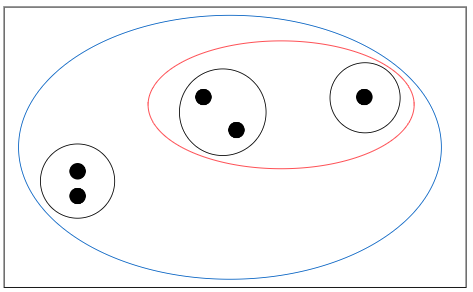
\includegraphics[width=8cm]{img/bab_2/hierarchi.png}
		\captionof{figure}{Hasil Hierarchical Clustering pada Objek}
		\label{fig:asd}
	\end{center}

	Pendekatan \textit{Agglomerative} dimulai dari setiap objek memiliki partisi masing-masing dan terpisah, kemudian algoritma mengukur nilai \textit{proximity matrix} setiap objek untuk menentukan berapa banyak penggabungan partisi lain yang perlu dilakukan. Proses dilakukan berulang kali dan jumlah partisi akan berkurang hingga tersisa satu partisi, satu partisi ini memiliki keseluruhan objek. Sedangkan pendekatan secara \textit{divisive} melakukan hal yang sama seperti \textit{Agglomerative} namun prosesnya terbalik yaitu dimulai dari satu partisi \cite{2C9}.

	\begin{center}
		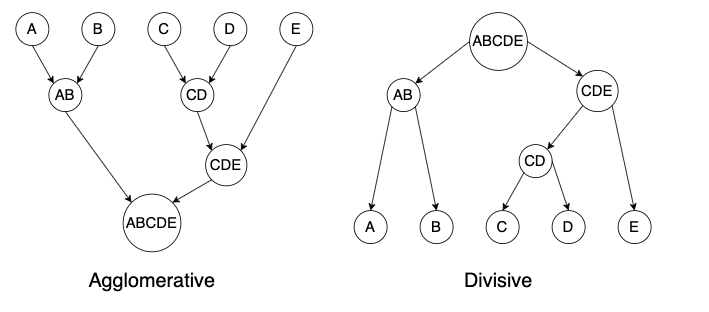
\includegraphics[width=12cm]{img/bab_2/agVSDiv.png}
		\captionof{figure}{Perbedaan Agglomerative dan Divisive}
		\label{fig:asd}
	\end{center}

	Ada beberapa metode untuk menentukan partisi terdekat yaitu dengan menghitung jarak maksimal antara objek partisi (complete lingkage), nilai rata-rata jarak(average lingkage) atau jarak minimum (single lingkage) \cite{3D3}. Proses untuk menghitung \textit{Hierarchical Agglomerative Clustering}(HAC) menghasilan stepwise matrix yang dapat digunakan untuk membuat dendogram. Proses ini menggunakan perbandingan jarak antar objek(X). Untuk mengabungkan hasil kumpulan jarak menggunakan algoritma linkage, hasil dari linkage digabungkan dan disimpan ke dalam array baru. Array yang baru(d) berisi jarak terbaru antar objek lainnya yang belum digabungkan. Proses berakhir ketika semua objek sudah terhitung keterhubungannya dari individu objek yang memiliki banyak partisi hingga menjadi satu partisi yang memiliki banyak objek \cite{09E}.
	
	\begin{center}
		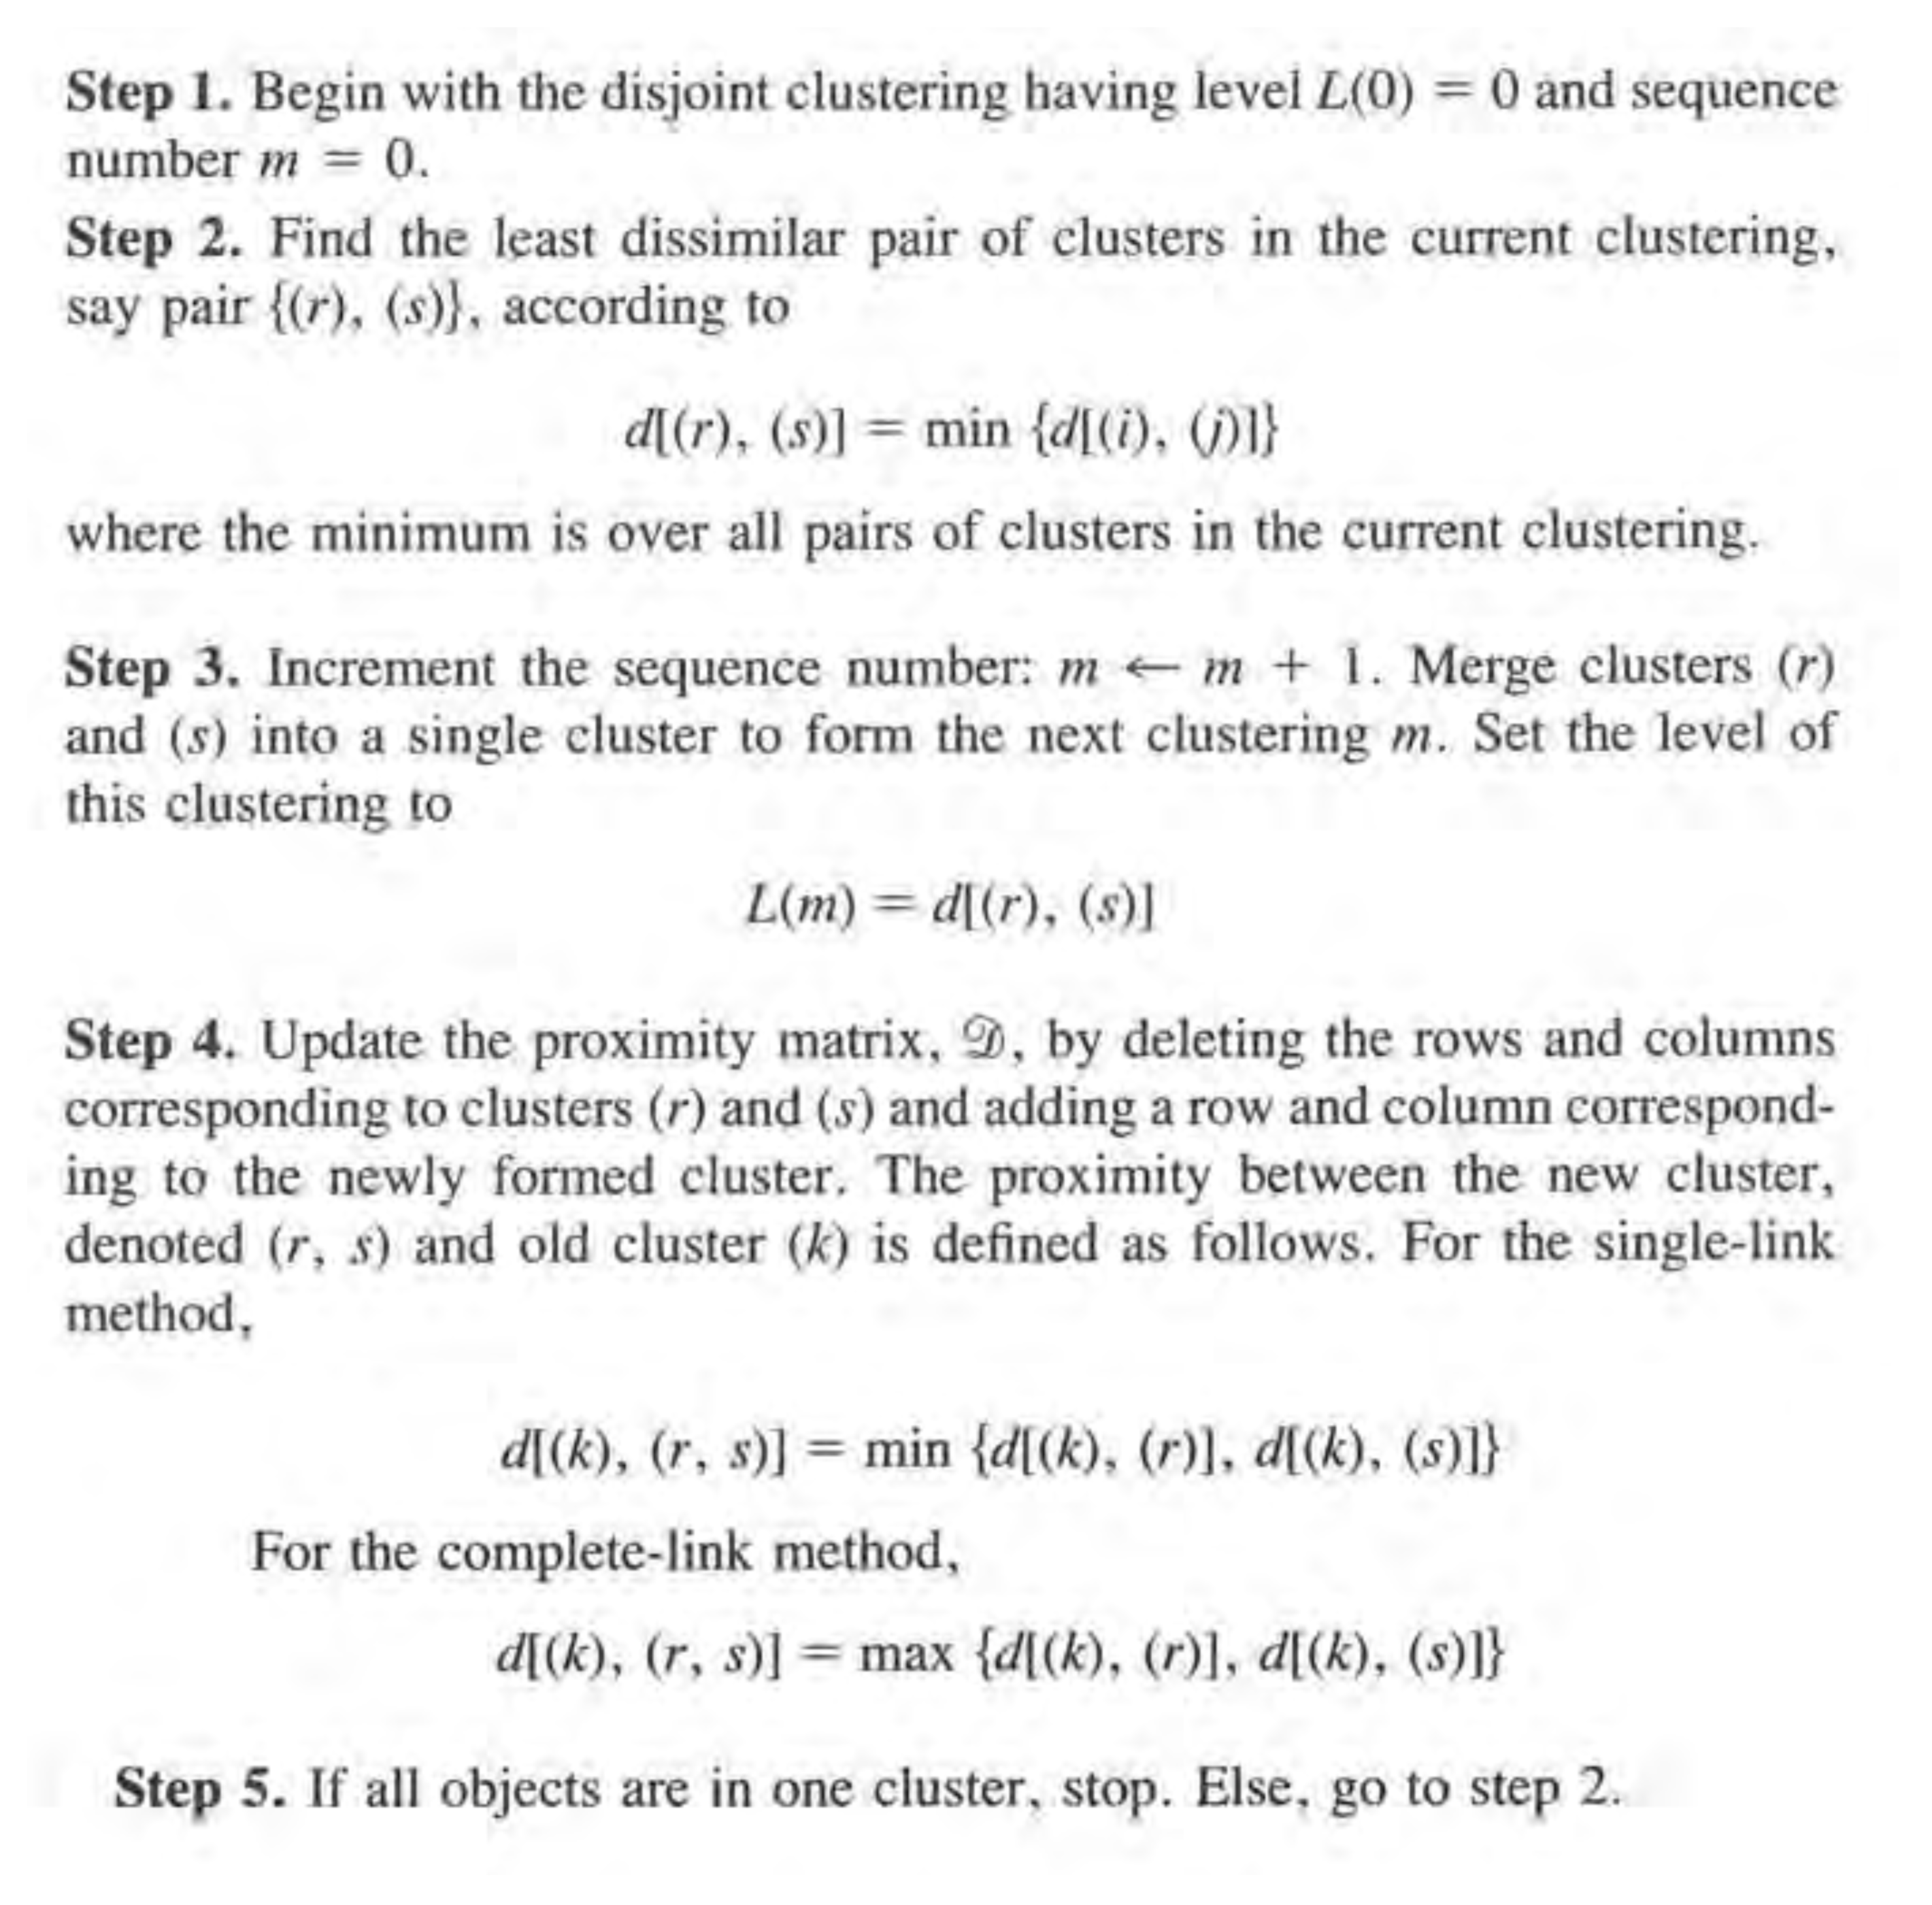
\includegraphics[width=12cm]{img/bab_2/algo_hac.png}
		\captionof{figure}{Algoritma \textit{Hierarchical Agglomerative Clustering} \cite{09E}}
		\label{fig:asd}
	\end{center}

	\item \textit{Partitional Clustering} \\
	\textit{Partitional} menggunakan pendekatan di mana diberikan sejumlah \textit{n} pola pada data dimensional, kemudian tentukan partisi dari pola menjadi beberapa \textit{cluster}. Pendekatan \textit{Hierarchical} populer digunakan dibidang biologi, sosial, dan ilmu perilaku karena keperluan untuk membentuk suatu taxonomi. Sedangkan \textit{Partitional} digunakan umumnya di aplikasi teknik. 

	\begin{center}
		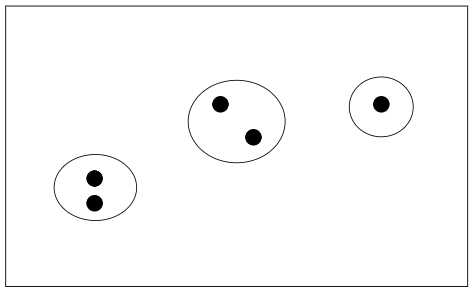
\includegraphics[width=8cm]{img/bab_2/partional.png}
		\captionof{figure}{Hasil Partitional Clustering pada Objek dengan n=3}
		\label{fig:asd}
	\end{center}

	Di mana satu partisi lebih penting, Metode \textit{Partitional} juga memiliki efisiensi dan kompresi yang cocok untuk data yang besar sehingga pola dalam \textit{cluster} memiliki kemiripan satu sama lain daripada pola dalam \textit{cluster} yang berbeda. Pemilihan nilai \textit{cluster} bisa ditentukan secara opsional, kriteria \textit{cluster} yang valid harus ditentukan seperti \textit{square-error} untuk menentukan apakah partisi yang dibuat optimal. Kriterianya sendiri bisa dibagi menjadi secara global atau lokal.  

\end{enumerate}	

\subsubsection{Pemilihan Partisi}
Untuk mengetahui apakah pengelompokan yang dihasilkan dari proses \textit{clustering} memiliki kualitas yang tepat maka perlu dilakukan evaluasi yang mempertimbangkan aspek \textit{microservice}.	
\begin{enumerate}[leftmargin=1.3cm]
	\item \textit{Structural and Behavioral Dependencies} \cite{5B1}\\
	Microservice dapat dilihat sebagi kumpulan dari suatu \textit{class} yang berkolaborasi satu sama lain untuk memberikan suatu fungsi. Hal ini dapat ditentukan dari kode program melalui nilai internal \textit{coupling}. Kolaborasi bisa ditentukan dengan nilai \textit{cohesion} dari jumlah data seperti atribut yang tidak tetap.

	\begin{equation}
		F O n e(M)=\frac{1}{2}(I n t e r C o u p(M)+I n t e r C o h(M))
	\end{equation}
	
	Nilai Internal Coupling dapat dihitung dari jumlah koneksi secara langsung atau tidak langsung melalui ketergantungan di antara \textit{class}(CoupP) dengan jumlah kemungkinan koneksi yang bisa terjadi di antara \textit{class} (NbPossiblePairs). Ketika dua \textit{class} semakin banyak menggunakan fungsi satu sama yang lain, maka semakin tinggi nilai kopelnya. 

	\begin{equation}
		I n t e r C o u p(M)=\frac{\sum C o u p P(P)}{N b P o s s i b l e P a i r s}
	\end{equation}
	
	Perbandingan nilai \textit{coupling} antara dua \textit{class} dihitung oleh fungsi CoupP, fungsi CoupP membagi jumlah \textit{call} yang terjadi(NbCals) antara 2 \textit{class}(C1,C2) dengan total \textit{call} yang dilakukan \textit{class} tersebut(TotalNbCalls).

	\begin{equation}
		C o u p P(C1,C2)={\frac{N b C a l s(C1,C2)+N b C a l s(C2,C1)}{T o t a l N b C a l l s}}
	\end{equation}	
	
	Perhitungan nilai \textit{coupling} eksternal, dilakukan sama dengan perhitungan nilai \textit{coupling} internal tapi yang membedakannya adalah hanya menghitung jumlah \textit{call} kepada \textit{class} eksternal.
	
	Untuk menghitung nilai \textit{cohesion} dapat dilakukan dengan menghitung jumlah interaksi \textit{class} di dalam partisi. Perhitungan ini dapat dihitung dengan fungsi InterCoh. InterCoh membagi antara jumlah \textit{call} yang terjadi di dalam \textit{class} (NbDirectConnections) dengan jumlah \textit{call} yang hanya memanggil \textit{class} di dalam partisinya sendiri (NbPossibleConnections).
	
	\begin{equation}
		I n t e r C o h(M)=\frac{N b D i r e c t C o n n e c t i o n s}{N b P o s s i b l e C o n n e c t i o n s}
	\end{equation}
	
	\item \textit{Data Autonomy Class} \cite{5B1}\\
	Salah satu karakteristik \textit{microservice} adalah memiliki data Autonomy. Sebuah \textit{microservice} dapat berdiri sendiri bila tidak memerlukan data dari \textit{service} lainnya. Dengan demikian semakin kecil pertukaran data antar \textit{service} maka semakin baik \textit{microservice}. Perhitungan dilakukan dengan mengukur nilai ketergantungan data antara \textit{class} dan ketergantungannya dengan \textit{class} external.
	
	\item \textit{Iter-Paritition Call Percentage}(ICP) \cite{ECD} \\
	Menghting jumlah persentase \textit{call} secara runtime antara 2 partisi di \textit{microservice}. Semakin kecil nilai ICP menunjukkan kurangnya interaksi antara partisi di mana merepresentasikan \textit{microservice} yang bagus.	
	
	\item Jumlah Interface \cite{ECD} \\
	Jumlah Interface/ Interface Number(IFN) menghitung jumlah interface yang ada di dalam \textit{microservice}. ifni adalah jumlah interface di dalam \textit{microservice} dan N adalah total interface di \textit{microservice}. Semakin kecil nilai IFN mengindikasikan rekomendasi \textit{microservice} yang lebih baik\\


\end{enumerate}	

\subsection{Teknologi dan \textit{Library}}
\subsubsection{\textit{Docker} \cite{docker}}
Docker adalah sebuah platform terbuka untuk \textit{container} yang dapat membuat \textit{container} dan mengelola container. Docker dapat memisahkan aplikasi dengan infrastruktur sehingga pengembangan aplikasi bisa berjalan dengan cepat. Dengan Docker, pengguna dapat mengelola infrastruktur sama seperti mengelola aplikasi.

Arsitektur Docker menggunakan arsitektur \textit{client}-server. Docker \textit{client} berkomunikasi dengan Docker daemon, yang melakukan pekerjaan seperti membangun, menjalankan, dan mendistribusikan docker containers. Docker \textit{client} dan daemon dapat berjalan disistem yang sama atau docker \textit{client} berhubungan dengan daemon melalui jaringan seperti REST API. 
\\
\subsubsection{\textit{PyCG} \cite{AD7}}
PyCG adalah tools analisis statik pada bahasa pemrograman Python. PyCG memiliki kemampuan untuk otomatis menemukan module untuk melakukan analisis lebih lanjut. PyCG bisa menghasilkan \textit{call graph} dari suatu kode baik file maupun dalam bentuk package.

PyCG juga memiliki presisi dan \textit{recall} yang tinggi bila dibandingkan dengan alat lainnya seperti Pyan dan Depends. PyCG sudah dievaluasi dengan projek lainnya baik kecil atau besar. Pendekatan PyCG modular , mudah dikembangkan lebih lanjut dan mencakup sebagian besar fungsionalitas Python.
\\
\subsubsection{\textit{Kong Gateway} \cite{kong}}
Kong Gateway adalah \textit{API Gateway} yang ringan, cepat, dan fleksibel serta kompatibel di Cloud. Dengan Kong Gateway pengguna dapat membuat automatisasi, desentralisasi aplikasi/service dan transisi ke \textit{microservice} dan memiliki kemampuan mengatur dan mengawasi API.

Kong Gateway memiliki Kong Manager yaitu graphical user interface (GUI). Di mana menggunakan Kong Admin API untuk mengatur Kong Gateway. Kong Manager dapat menambahkan rute dan \textit{service} baru, mengaktifkan dan mematikan plugins, membuat grup untuk tim, dan penmantauan serta pengecheckan status \textit{service}. Plugins dapat menambahkan fitur pada Kong seperti rate limiting untuk mengkontrol jumlah request yang dikirimkan ke suatu servie dan pengaturan cache.
\\
\subsubsection{\textit{inspect} \cite{inspect}}
Inspect adalah library bawaan dari python , di mana library ini memberikan fungsi untuk mengetahui informasi tentang object yang sedang hidup seperti module,class, method, fungsi, traceback, frame object, dan kode object. Terdapat 4 bagian pada library ini yaitu pengecheckan tipe data, mendapatkan kode program, inpeksi \textit{class} atau fungsi, dan memeriksa interpreter stack.

Module yang digunakan pada tugas akhir ini:
\begingroup
\setlength{\LTleft}{-20cm plus -1fill}
\setlength{\LTright}{\LTleft}
\begin{small}
	\begin{longtable}{|p{3cm}|p{5cm}|p{4.5cm}|}
		\caption{Daftar Metode dan Fungsi inspect}\\
		\hline
		\textbf{Nama} & \textbf{Keterangan} & \textbf{Atribut}\\
		\endfirsthead
		
		\hline
		    inspect.getmembers
		  &  untuk mendapatkan member dari sebuah objek seperti \textit{class} atau module
		  & object = objek yang ingin didapatkan membernya\\
		\hline 
		    inspect.ismodule
		  & untuk mengetahui apakah objek adalah sebuah module
		  & object = objek yang ingin dilakukan pengecekan\\
		\hline  
		\hline
		    inspect.isclass
		  & untuk mengetahui apakah objek adalah sebuah \textit{class}
		  & object = objek yang ingin dilakukan pengecekan\\
		\hline  
	\end{longtable}
\end{small}
\endgroup

\subsubsection{\textit{SciPY} \cite{scipy}}
SciPY adalah koleksi algoritma matematika yang cocok dengan ekstensi NumPY di Python. SciPy memiliki module algoritma clustering yang dapat digunakan dan dapat dilakukan pemilihan metode yang mungkin dibutuhkan. Proses Perhitungan yang dilakukan SciPy sudah di optimalisasi dan efisien.

Module algoritma yang digunakan pada tugas akhir ini:
\begingroup
\setlength{\LTleft}{-20cm plus -1fill}
\setlength{\LTright}{\LTleft}
\begin{small}
	\begin{longtable}{|p{3cm}|p{5cm}|p{4.5cm}|}
		\caption{Daftar Metode dan Fungsi SciPy}\\
		\hline
		\textbf{Nama} & \textbf{Keterangan} & \textbf{Atribut}\\
		\endfirsthead
		
		\hline
		 	single
		  & melakukan pengelompokan dengan nilai minimal atau nilai terdekat pada matriks kedekatan
		  & y = matriks kedekatan \\
		\hline  
		 average
		  & melakukan pengelompokan dengan nilai rata-rata jarak pada matriks kedekatan
		  & y = matriks kedekatan \\
		\hline  
		complete
		  & melakukan pengelompokan dengan nilai maximal atau nilai terjauh pada matriks kedekatan
		  & y = matriks kedekatan \\
		  \hline  
		dendogram
		  & mengilustrasikan dendogram dari \textit{cluster} yang terbentuk di matriks linkage
		  & Z = matriks linkage  \\
		\hline  
	\end{longtable}
\end{small}
\endgroup


\section{Tinjauan Studi}
\par Pada Tabel \textbf{2.1} diberikan penjelasan mengenai studi yang terkait dalam tugas akhir:

\begingroup
\setlength{\LTleft}{-20cm plus -1fill}
\setlength{\LTright}{\LTleft}
\begin{small}
	\begin{longtable}{|p{3cm}|p{3.5cm}|p{3cm}|p{3.5cm}|}
		\caption{\textit{State of the Art}}\\
		\hline
		\textbf{Jurnal} & \textbf{Rumusan Masalah} & \textbf{Metode} & \textbf{Hasil}\\
		\endfirsthead

		\hline
		A. Selmadji, A.-D. Seriai, H. L. Bouziane, R. Oumarou Mahamane, P. Zaragoza, and C. Dony   (2020). "\textbf{From monolithic architecture style to Microservice one based on a semi-automatic approach}" \cite{5B1} &
		Terdapat aplikasi monolitik yang tidak beradaptasi di \textit{cloud} ataupun \textit{DevOps} sehingga harus dimigrasi ke \textit{microservice} &
		Analisis kode program dan mencari hubungan dalam \textit{class}-nya  &
		Identifikasi Microservice yang dibuat memiliki hasil yang memuaskan karena mempertimbangkan karakteristik microservice
		\\

		\hline
		Chaitanya K. Rudrabhatla. (2020). "\textbf{Impacts of Decomposition Techniques on Performance and Latency of Microservices.}"  \cite{6C1} &
		Bagaimana dampak performa dalam menentukan batasan antar \textit{service}  &
		Melakukan perbandingan antara pendekatan DDD, Normalized Entity Relationship, dan Hybrid &
		Teknik DDD lebih baik dalam dekomposisi namun teknik Hybrid dengan mempertimbangkan fungsionalis dan transaksi yang terjadi memiliki performa lebih baik.
		\\

		\hline
		A. K. Kalia, J. Xiao, R. Krishna, S. Sinha, M. Vukovic, and D. Banerjee (2021). "\textbf{Mono2micro: A practical and effective tool for decomposing monolithic Java applications to microservices}" \cite{8EA} &
		Bagaimana pendekatan Mono2Micro dengan cara dekomposisi lainnya dan bagaimana tanggapan praktisi&
		Menggunakan hierarchical spatio-temporal decomposition  yang menyimpan kondisi program secara dinamik berdasarkan eksekusi proses bisnis  &
		Hasil rekomendasi \textit{microservice} dapat membantu penerapan pola \textit{strangle} , partisi yang dihasilkan sesuai dengan fungsi bisnis
		\\
		
		\hline
		Khaled Sellami, Mohamed Aymen Saied, and Ali Ouni. (2022). "\textbf{A Hierarchical
		DBSCAN Method for Extracting Microservices from Monolithic Applications}" \cite{ECD} &
		Bagaimana mengotomatisasi proses migrasi aplikasi monolitik ke microservice?  &
	    Menggunakan DBSCAN(Density-based Clustering) yang menghasilkan rekomendasi \textit{microservice}  &
		Berhasil membuat \textit{microservice} yang lebih \textit{cohesion} dan memiliki interaksi yang lebih sedikit. 
		\\
		\hline
	\end{longtable}
\end{small}
\endgroup
Pada penelitian yang dilakukan oleh  A. Selmadji, A.-D. Seriai, H. L. Bouziane, R. Oumarou Mahamane, P. Zaragoza, dan C. Dony \cite{5B1}, penelitian melakukan identifikasi \textit{microservice} dari aplikasi Monolitik berbasis Object-Oriented(OO). Identifikasi  dimulai dari membuat partisi dari proses pengelompokan untuk menemukan \textit{microservice} yang bagus dengan memperhitungkan karakteristik dari \textit{microservice} seperti berdasarkan struktural dan perilaku ketergantungan \textit{microservice} serta \textit{Data Autonomy}. Untuk mengevaluasi hasil identifikasi yang dibuat yaitu dengan menggunakan kode program yang sudah menjadi \textit{microservice} dan kemudian membandingkannya antara rekomendasi dan yang sebenarnya. 

Hasil dari penelitian tersebut adalah identifikasi \textit{microservice} terbaik bisa dilakukan melalui algoritma gravity center dengan keseluruhan kode program. Penggunaan Fungsi untuk mengetahui \textit{microservice} terbaik dapat dilakukan hanya dengan cara struktural tanpa harus mempertimbangkan \textit{data autonomy}.

Pada penelitian yang dilakukan oleh Chaitanya K. Rudrabhatla \cite{6C1}, penelitian melakukan perbandingan latensi antara pemilihan dekomposisi. Peneliti menggunakan aplikasi yang dibuat dengan Spring Boot Java. Dari hasil evaluasi diketahui dekomposisi dengan domain driven desain(DDD)  memiliki performa lebih baik daripada pendekatan melalui entitas. Namun dengan pendekatan hybrid/campuran performa antara domain driven memiliki kesamaan sehingga diperlukan transaksi yang komplex untuk melihat perbedaan

Pada penelitian yang dilakukan oleh A. K. Kalia, J. Xiao, R. Krishna, S. Sinha, M. Vukovic, dan D. Banerjee \cite{8EA}, peneliti menggunakan Mono2Micro untuk melakukan dekomposisi aplikasi monolitik Java menjadi \textit{microservice}. Kemudian menggunakan metrik untuk mengevaluasi apakah \textit{microservice} yang dibuat oleh Mono2Micro efektif. Peneliti menggunakan 5 metrik untuk mengukur efektifitas yaitu  secara Structural Modularity(SM), Indirect Call Patern(ICP), Business Context Purity(BCP), jumlah Interface(IFN), dan Non-Extreme Distribution(NED) serta ada survey kepada praktisi mengenai penggunaan Mono2Micro

Hasil dari penelitian menunjukkan bahwa penggunaan Mono2Micro efektif dalam melakukan dekomposisi dan dapat memberikan keuntungan bagi pengembang karena bisa membantu pengembang untuk melihat partisi lainnya. Metrik yang dihasilkan dari Mono2Micro memiliki hasil yang bagus di antara 5 metrik tersebut, namun diperlukan penelitian lebih lanjut pada kasus tingginya nilai SM menyebabkan tingginya nilai NED.

Pada penelitian yang dilakukan oleh Khaled Sellami, Mohamed Aymen Saied, and Ali Ouni \cite{ECD}. Penelitian menggunakan Algoritma Hierarchical DBSCAN dengan analisis statik kode program untuk mendapatkan sekumpulan \textit{service} yang bisa kandidat \textit{microservice}.  Peneliti menggabungkan nilai struktural dan nilai semantik analisis untuk menentukan kedekatan suatu \textit{class} dengan \textit{class} lainnya.
Hierarchical DBSCAN. Prose evaluasi menggunakan perbandingan antara \textit{microservice} \textit{service} yang sudah diekstraksi sebelumnya oleh pengembang. 

Hasil dari penelitian menunjukkan pendekatan hierarchical clustering dapat melakukan dekomposisi aplikasi monolitik dengan analisis statik. Microservice yang didekomposisi memiliki nilai \textit{cohesion} yang lebih baik di dalam \textit{microservice} dan  jumlah interaksi antar \textit{microservice} lebih sedikit.
\\

\section{Tinjauan Objek}
Pada bagian ini akan dijelaskan mengenai objek dan aplikasi terkait yang akan digunakan dalam tugas akhir ini. Object yang digunakan adalah sebuah aplikasi Enterprise Resource Planning yang di deploy secara monolitik, yaitu Odoo.

Odoo merupakan aplikasi bisnis open source yang dapat mencakup semua kebutuhan perusahaan seperti CRM(Customer Relationship Management), eCommerce, akuntansi, inventaris, POS(Point of Sales), manajemen proyek dan lainnya. Aplikasi ini flexibel karena bisa dikembangkan lebih lanjut bila diperlukan dan bisa diubah karena memiliki lisensi source code yang terbuka \cite{odoo}. 

Sebelum Odoo terdapat OpenERP, di mana OpenERP memiliki arsitektur monolitik. Pada versi OpenERP ke 7, karena banyaknya pengembangan fitur yang membuat waktu pengembangan menjadi lama dan sulit. OpenERP melakukan migrasi menjadi arsitektur SOA dan berganti nama menjadi Odoo \cite{5FA}.

Arsitektur yang digunakan pada Odoo yaitu three-tier arsitektur di mana tampilan, aturan bisnis dan tempat penyimpanan data memiliki lapisan terpisah. Dengan tujuan memudahkan dan mempercepat pengembang untuk melakukan modifikasi aplikasi tanpa harus mengganggu lapisan lainnya \cite{odoo}.

\begin{center}
	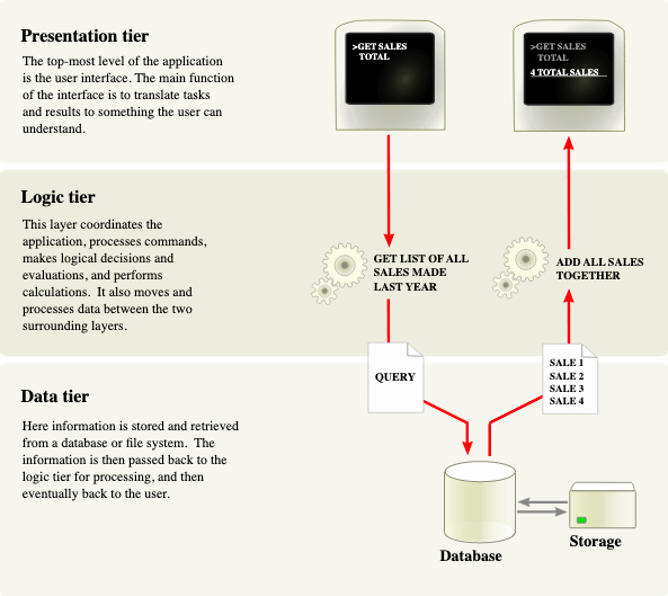
\includegraphics[width=8cm]{img/arsitekturOdoo.PNG}
	\captionof{figure}{Arsitektur Odoo \cite{odoo}}
	\label{fig:asd}
\end{center}

Pada tingkatan paling atas yaitu tampilan(presentation tier), tampilan ini yang akan berinteraksi langsung dengan pengguna yang menggunakan aplikasi. Tampilan ini dibangun dengan teknologi web yaitu HTML5, Javascript, dan CSS. Tingkatan dibawahnya yaitu aturan bisnis(logic tier) yang berisi instruksi yang memproses data dan memberikan tanggapan dari interaksi kepada pengguna. Aturan pada Odoo hanya ditulis dalam bahasa pemrograman Python. Sedangkan pada tingkat paling bawah adalah tempat penyimpanan menggunakan DBMS(Database Management System), Odoo hanya bisa mendukung \textit{database} PostgreSQL \cite{odoo}.

Struktur \textit{module} pada kode program di Odoo versi 16 yaitu ada folder debian dan setup yang menangani bagaimana aplikasi Odoo diinstall di berbagai platform. Folder doc berisi mengenai dokumentasi dan hak cipta. Folder odoo merupakan module utama aplikasi odoo tanpa ada module ini maka aplikasi tidak dapat dijalankan. Folder addons berisi module yang memiliki aset serta bisa diganti atau dihilangkan sesuai kebutuhan. File seperti odoo-bin untuk memulai aplikasi odoo, requirements.txt berisi library python yang dibutuhkan aplikasi odoo.

\begin{center}
	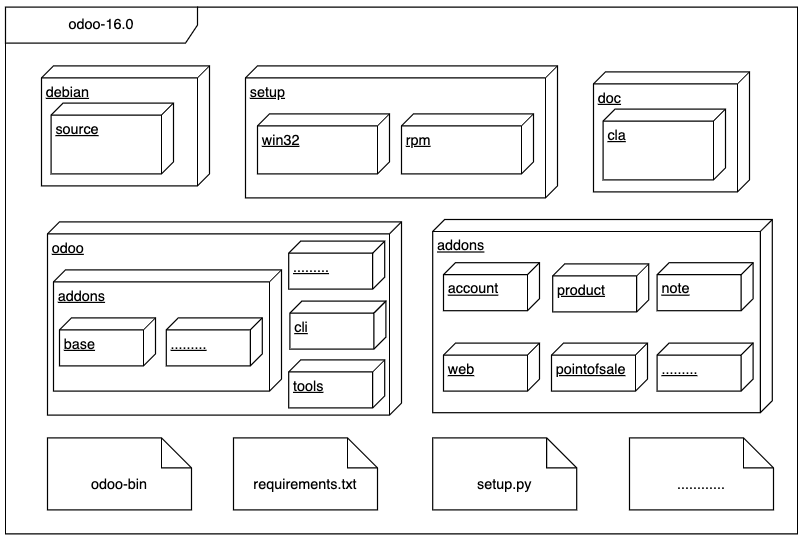
\includegraphics[width=14cm]{img/bab_2/folder_odoo.png}
	\captionof{figure}{Struktur Repository Odoo }
	\label{fig:asd}
\end{center}

Odoo memiliki struktur kode yang dibentuk sebagai module untuk setiap fiturnya. Sehingga dari sisi server dan \textit{client} memiliki hubungan yang disatukan menjadi satu paket tersendiri. Di mana module adalah koleksi dari fungsi dan data untuk menyelesaikan satu tujuan. Modul pada Odoo bisa ditambahkan, diganti, diubah untuk menyesuaikan kebutuhan bisnis. Di mana pada pengguna module dilambangkan dengan nama Apps, tetapi tidak semua module adalah Apps. Modules juga bisa direfrensikan sebagai addons \cite{odoo}. 

\begingroup
\setlength{\LTleft}{-20cm plus -1fill}
\setlength{\LTright}{\LTleft}
\begin{small}
	\begin{longtable}{|p{2.5cm}|p{6cm}|p{4.5cm}|}
		\caption{Komposisi dari Module pada aplikasi Odoo \cite{odoo}:}\\
		\hline
		\textbf{Elemen} & \textbf{Keterangan} & \textbf{Contoh}\\
		\endfirsthead
		
		\hline
		    Business Objects
		  & Object yang akan digunakan di module di mana setiap attribute secara otomatik dipetakan ke kolom \textit{database} dengan ORM
		  & File python yang memiliki \textit{class}\\
		\hline  
		Objects Views
		  & Menangani bagaimana data ditampilkan di pengguna. Seperti visualisasi form, list, kanban dan lainnya
		  & Berupa file XML dengan struktur yang sudah ditentukan Odoo\\
		\hline
		Data Files
		  & Mengelola bagaimana model data seperti laporan, konfigurasi data, data contoh dan lainnya
		  & Berupa file XML atau CSV\\
		\hline
		Web Controllers
		  & Menangani permintaan dari browser/client
		  & File python yang memiliki \textit{class} namun merupakan turunan dari \textit{class} odoo.http.Controller\\
		\hline
		  Static Web Data
		  & File yang digunakan hanya ditampilkan kepada \textit{client} di website
		  & File gambar, File CSS, dan File JavaScript\\
		 \hline  
	\end{longtable}
\end{small}
\endgroup
Terdapat 2 jenis addons yaitu addons base dan addons. Yang membedakannya addons base harus ada di setiap aplikasi Odoo bila tidak ada aplikasi tidak dapat berjalan sedangkan addons bisa diganti sesuai keperluan bisnis. Pengelolaan \textit{database} dilakukan secara otomatis oleh ORM internal Odoo, Odoo memiliki framework yang bisa digunakan untuk menambahkan atau mengelola fitur atau addons. 

Tabel yang terbentuk pada konfigurasi umumnya bisa mencapai ±566 tabel bila semua module di install sementara itu jumlah tabel tanpa ada module terinstall adalah 99 tabel. Dari tabel tanpa ada module bisa diidentifikasi 27 tabel utama yang digunakan pada aplikasi. Berikut adalah diagram dari \textit{database} aplikasi Odoo, dengan attribute yang ditampilkan hanya sebuah key dari tabel. Nama depan tabel yang berinisial 'ir' artinya information repository dan 'res' artinya resource. Perbedaannya adalah 'res' menyimpan informasi yang digunakan dalam proses bisnis sedangkan 'ir' menyimpan informasi mengenai kebutuhan internal aplikasi.
 
\begin{center}
	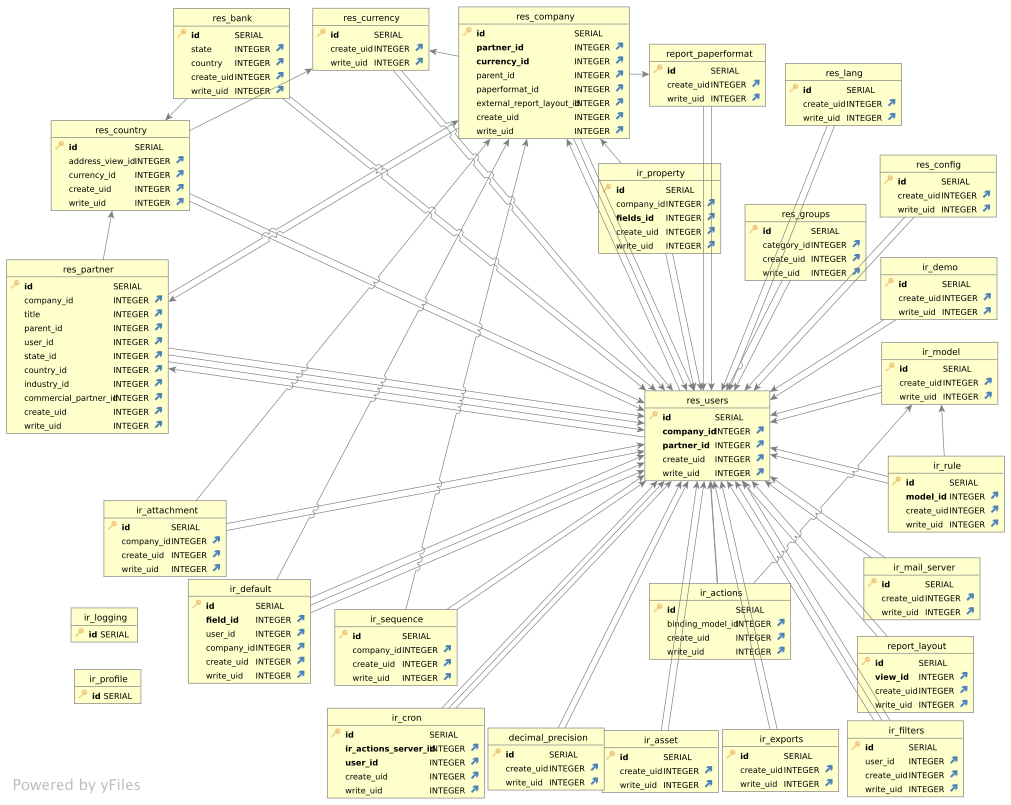
\includegraphics[width=14cm]{img/OdooCoreERD.png}
	\captionof{figure}{Skema Database Odoo }
	\label{fig:asd}
\end{center}



